%\ctparttext{\color{black}\begin{center}
%		Esta es una descripción de la parte de informática.
%\end{center}}

%\part{Parte de informática}
\chapter{Quantum Mechanics Model}


Quantum Mechanics are a mathematical framework in which quantum physics are developed. In this section, we will develop a quantum mechanics model in order to understand quantum computing. The Quantum Postulates will be our guidance. They provide a connection between the physical world and the mathematical formalization. We will provide context and formalization for each postulate, so both the mathematical precision and intuition notions are developed at the same time. This development is based on \cite{Nielsen2002}, \cite{Manzano2020} and \cite{Bayens2019}.


\section{Postulate 1: State Space}


The first postulate sets the environment in which we will operate: The State Space. It will be a Hilbert space associated to a physicial system. Let us rigorously define the necessary concepts using the Bra-ket notation. We will start by revisiting the required linear algebra.


\subsection{Bra-ket notation}


Let $V$ be a complex vector space. That is, a vector space over $\C$. We will restrict our study to finite complex vector spaces. If $z$ is a vector in $V$, we will denote its coordinates either as $z = (z_1, z_2, \dotsc, z_n)$ or by column notation:

$$ z = 
\begin{pmatrix}
	z_1\\
	z_2 \\
	\vdots \\
	z_n
\end{pmatrix}
$$

Since $V$ is a vector space we have two basic operations: (vector) addition and scalar multiplication.

In quantum mechanics, the usual notation is the Dirac's, also known as \emph{bra-ket} notation. In this context, vectors in a complex vector space are denoted as $|\varphi\ra$ and are known as \emph{kets}. The only exception to this is the zero vector, which will be denoted as $0 = (0, \dotsc, 0)$ instead of $|0\ra$ since $|0\ra$ will be used as something completely different. A \emph{vector subspace} $W$ of $V$ is a subset of $W$ closed for addition and scalar multiplication.

A \emph{base} of a vector space is a set of vectors $|v_1\ra, \dotsc, |v_n\ra$ such that they are linearly independent and any given vector $|v\ra$ can be written as a linear combination of them: $|v\ra = \sum_{i=1}^n \alpha_i|v_i\ra$. The \emph{dimension} of a vector space is the number of elements in any of its bases, which is independent from the chosen base.

\begin{definition}
	Given two complex vector spaces $V$ and $W$, a \emph{linear operator} is an application $M: V \rightarrow W $ that is linear in its inputs:
	
	$$ M \Big( \alpha |u\ra + \beta |w\ra \Big) = \alpha M (|u\ra) + \beta M (|w\ra) $$
\end{definition}

If $V$ to $W$ have dimensions $n$ and $m$ respectively, there is a bijection between the operators from $V$ to $W$ and the $n$ by $m$ matrices. Given an operator $M$, the obtained matrix $M'$ is called the \emph{matrix representation} of the linear operator. Furthermore, $M(|u\ra) = M' \cdot |u\ra$, so we usually denote the linear operator and its matrix representation by the same letter, and $M(|u\ra)$ simply as $M|u\ra$.

We will usually refer to linear operators simply as \emph{operators}.


\subsection{Inner product and Hilbert Spaces}


Let us define another operation within the complex vector spaces.

\begin{definition}
	Let $V$ be a complex vector space. An inner product $\la \cdot | \cdot \ra: V^2 \rightarrow \C$ is a function such that:
	
	\quad 1) $\la \cdot | \cdot \ra$ is sesquilinear. That is,
	
	\qquad 1.1) $\la \cdot | \cdot \ra$ is conjugate symmetric: for all $u,v$ in $V$, $\la u | v \ra = \overline{\la v | u \ra}$.
	
	\qquad 1.2) $\la \cdot | \cdot \ra$ is linear on the second variable: for all $u,v,w$ in $V$ and $\alpha, \beta$ in $\C$:
	
	$$ \la u  | \alpha v + \beta w \ra = \alpha \la u | v \ra + \beta \la u | w \ra $$
	
	\quad 2) $\la \cdot | \cdot \ra$ is definite positive. That is, for all $u$ in $V$, $\la u | u \ra \geq 0$ and $\la u | u \ra = 0 \Longleftrightarrow v = 0$.
\end{definition}

Given this properties it can easily be proven that $\la \cdot | \cdot \ra$ is also conjugate linear on the first variable. That is, for all $u,v,w$ in $V$ and $\alpha, \beta$ in $\C$:

$$ \la \alpha u + \beta v  | w \ra = \overline{\alpha} \la u | w \ra + \overline{\beta} \la v | w \ra $$

We will sometimes denote the inner product $\la \cdot | \cdot \ra$ as $( \cdot , \cdot )$ to simplify notation.

Two vectors are said to be \emph{orthonormal} if their inner product is zero. We define the norm of a vector $|v\ra$ by:

$$\parallel |v\ra \parallel \ = \sqrt{ \la v|v\ra }$$

A \emph{unit vector} is a vector $|v\ra$ such that $\parallel |v\ra \  \parallel \ = 1 $. We also say that $|v\ra$ is \emph{normalized}, and we can normalize any vector except the zero vector by dividing it by its norm.

A base $|v_1\ra, \dotsc, |v_n\ra$ is said to be \emph{orthonormal} if every vector is a unit vector and they are pairwise orthogonal. That is, $\la v_i|v_j\ra = \delta_{ij}$ where

\[
\delta_{ij} = 
\begin{cases}
	1 & \text{if } i = j  \\
	0 & \text{if } i \neq j
\end{cases}
\]

\begin{definition}
	An \emph{inner product space} is a vector space with an associated inner product. A \textbf{Hilbert Space} is an inner product space that is also complete.
\end{definition}

Hausdorff's Theorem states that every finite normed space is complete, therefore every finite inner product space over $\C$ is a Hilbert space \cite{Paya2020}. Again, by Hausdorff's theorem, we know that every $n$ dimensional Hilbert space is isomorphic to $\C^n$. Thus, $\C^n$ is the canonical $n$ dimensional Hilbert space. Our study will be focused on these spaces.

Let $\alpha = a + i \cdot b\in \C$. We define the \emph{conjugate}, $\bar \alpha$, as $\bar \alpha = a - i \cdot b$. The canonical inner product in $\C^n$ is:

$$ \la u|v \ra \ = \sum_{i=1}^n \overline{u_i}v_j $$

where $u = (u_1, \dotsc, u_n)$ and $v = (v_1, \dotsc, v_n)$, for every $u,v$ in $\C^n$.


\subsection{Postulate 1 statement}


The reader should be familiar by now with the notation and the necessary linear algebra to formulate the first postulate.

\begin{postulate}
	Associated to any isolated physical system is a complex vector space with an inner product (that is, a Hilbert space) known as the \emph{state space} of the system. The system is completely described by its \emph{state vector}, which is a unit vector in the system’s state space.
\end{postulate}

An important concern with this postulate is that it does not tell us which is the state space of a given system, nor its state vector. Although up to this point we cannot formally assure this, in quantum computing the state space will be fixed: $\C^{2^n}$ for an n-qubits system. Our evolving state vector will be a vector $2^n$-vector.

Let us start by modulating a simpler system: a single qubit system.

\begin{definition}
	A state vector of the state space $\C^{2}$ is called a \textbf{qubit}. Thus, $\C^{2}$ may be called a single qubit state space.
\end{definition}

Suppose $|0\ra$, $|1\ra$ form an orthonormal basis of a 2-dimensional Hilbert space. Then, any state vector in this state space may be described as:

$$ |\varphi\ra = \alpha|0\ra + \beta|1\ra $$

where $\alpha,\beta$ are complex numbers called \emph{amplitudes}. Thus, the condition that $|\varphi\ra$ is a unit vector, $\la\varphi|\varphi\ra = 1$ is equivalent to $|\alpha|^2 + |\beta|^2 = 1$. This is known as the \emph{normalization condition}.

We will always think of $|0\ra$, $|1\ra$ as a previously fixed orthonormal base. A linear combination of state vectors $\sum_i a_i |\varphi_i\ra$ is called a \emph{superposition} of the states $|\varphi_i\ra$ with amplitudes $a_i$ respectively. For example, the state

$$ \frac{|0\ra - |1\ra}{\sqrt 2} $$

is a superposition of the states $|0\ra$ and $|1\ra$ with amplitudes $1/\sqrt 2$ and $-1/\sqrt 2$ respectively.


\subsection{Quantum Computation Perspective: The Quantum Bit}


The bit is the minimum measure of information on classical computation and classical information theory. Everything in these fields is built from scratch based on bits. Likewise, quantum computing and quantum information theory are built upon the \textbf{qubit}.

We have reached the qubit definition from quantum physics and pure mathematics, describing the qubit as a mathematical object independent of its physical implementation. By describing them as mathematical entities we will be able to explore their properties mathematically without having to worry about the physics underneath.  This allows us to construct the quantum computing and quantum information theories independently of the physical implementation.

So, intuitively, what is a qubit? Just like the classical bit, a qubit has a state. For the bit, the two only possible states are either $0$ or $1$. A qubit can take the states $|0\ra$ and $|1\ra$ -corresponding to the classical states $0$ and $1$- or it can be in a \emph{linear combination} of them:

$$ |\varphi\ra = \alpha |0\ra + \beta |1\ra $$

Where $\alpha$ and $\beta$ are complex numbers. Thus, we can describe a qubit as a vector in a two-dimensional complex Hilbert space (the canonical $\C^{2}$), where $|0\ra$ and $|1\ra$ form an orthonormal basis called the \emph{computational basis}. $|0\ra$ and $|1\ra$ will be called \emph{computational basis states}.

At this point, the reader may ask themselves if a qubit may even physically exist, not just as a mathematical entity. After all, the first postulate states that given a \emph{physical system}, there is an associated state space and vector states that describe the system. However, we define a qubit from state space ($\C^{2}$) without considering a physical system. 

The answer is positive: there are numerous physical systems such that their associated state spaces are ($\C^{2}$). Thus, modeling a qubit. More intuitive examples are provided in section \ref{qubit-examples} and precise physical implementations are briefly discussed in section [TODOref].


\section{Postulate 2: Measurement}


The second postulate describes how states are 'measured', that is, how an outside observer may look inside the system. In classical physics, consider a simple system of a moving particle. 'Measuring' would be recording, for instance, the particle mass and speed at a given time. That is, someone \textbf{outside} the system would look \textbf{into} the system to record some information. Lastly, in the classical computation model measuring a bit is simply retrieving its content.

In quantum physics, measuring has some unexpected and sometimes counter-intuitive properties. Let us provide some linear algebra context before formulating the second postulate.


\subsection{Outer product}


\begin{definition}
	Let $V, W$ be two vector spaces and $|v\ra \in V, |w\ra \in W$. We define the \emph{outer product} between $|v\ra$ and $|w\ra$, $|w\ra\la v|$, as the only linear operator such that for any $|v'\ra \in V$, 
	
	$$ (|w\ra\la v|) \ |v'\ra = |w\ra\la v|v'\ra = \la v|v'\ra |w\ra$$
\end{definition}

These identities provide a dual interpretation: the already known product of a complex value $\la v|v'\ra$ with a vector $|w\ra$, and the application of the new operator, the outer product $|w\ra\la v|$ to the vector $|v'\ra$. The outer product is defined so that this duality occurs.

Let us consider linear combinations of outer products. By definition, $\sum_i a_i |w_i\ra\la v_i|$ is the operator that transforms $|v'\ra$ into $\sum_i a_i |w_i\ra\la v_i|v'\ra = \sum_i a_i \la v_i|v'\ra |w_i\ra$.

The most important result concerning outer products is the \emph{completeness relation}:

\begin{proposition}[Completeness relation]
	Let $|i\ra$ be any orthonormal basis of a finite vector space $V$. Then:
	
	$$ \sum_i |i\ra\la i| = I $$
\end{proposition}

\begin{proof}
	Let $|v\ra \in H$. $|v\ra$ can be expressed as $ \sum_i v_i |i\ra$ for some complex numbers $v_i$. Notice that $\la i|v\ra = v_i$. Therefor:
	
	$$|v\ra = \sum_i v_i |i\ra = \sum_i \la i|v\ra |i\ra = \sum_i |i\ra\la i|v\ra = \bigg( \sum_i |i\ra\la i|\bigg) |v\ra$$
	
	Since $|v\ra$ was arbitrary, this proves that $ \sum_i |i\ra\la i | = I $.
\end{proof}

\begin{corollary}[Cauchy-Schwarz inequality]
	For any two vectors $|v\ra, |w\ra$ in a Hilbert space,
	
	$$|\la v|w\ra|^2 \leq \la v|w\ra\la w|w\ra$$
	
	where the equality occurs if and only if $|v\ra$ and $|w\ra$ are linearly dependant
\end{corollary}
\begin{proof} 
	We provide a proof supposed that our Hilbert space is finite.
	
	Let $|v\ra, |w\ra$ be two vectors of a finite Hilbert space $H$. Since $H$ is finite, using the Gram-Schmidt procedure we may obtain a basis $|i\ra$ where the first vector is $|w\ra / \sqrt{\la w|w\ra}$. Using the completeness relation $\sum_i |i\ra \la i| = I$:
	
	$$\la v|v\ra \la w|w\ra = \la v|I|v\ra \la w|w\ra = \la v| \sum_i (|i\ra \la i|) |v\ra \la w|w\ra = \sum_i \la v|i\ra \la i|v\ra \la w|w\ra $$
	
	The sum of a list of positive numbers is obviously greater than its first element, so:
	
	$$ \sum_i \la v|i\ra \la i|v\ra \la w|w\ra \geq  \frac{\la v|w\ra \la w|v\ra}{\la w|w\ra} \la w|w\ra = \la v|w\ra \la w|v\ra  = | \la w|v\ra |^2 $$
	
	Lastly, the equality occurs if and only if $\la v|i\ra = 0$ for every $|i\ra \neq |w\ra / \sqrt{\la w|w\ra}$. But since $|i\ra$ is a base, this means $|v\ra$ and $|w\ra$ are linearly dependent.	
\end{proof}


\subsection{Unitary and Hermitian operators}


Another way of looking at the inner product is the \emph{adjoint}.

\begin{definition}
	Let $A$ be an operator between $\C^n$ and $\C^m$, finite dimensional Hilbert spaces. That is, $A \in \mathcal{M}_{n{\times}m}(\C)$. Then, its \emph{adjoint} or \emph{conjugate transpose} $A^\dagger$ is defined by:
	
	$$ (A^\dagger)_{ij} = \bar A_{ji} $$
\end{definition}

If $|v\ra$ is a vector, we can compute its adjoint by seeing it as a matrix. By convention, we will denote $|v\ra^\dagger = \la v|$. Adjoints of vector are usually called \emph{bras}, making given sense to the \emph{bra-ket} notation since $\la v| \cdot |v\ra = \la v|v\ra$, where $\cdot$ denotes the dot product.

Some useful algebraic identities associated to adjoints are:

\begin{itemize}
	\item Given an operator $A \in \mathcal{M}_{n}(\C)$, $A^\dagger$ is the only operator such that for any two vectors $|u\ra, |v\ra \in \C^n$: $( |u\ra, A|v\ra) = ( A^\dagger |u\ra, |v\ra)$
	\item For any two operators $A,B$, $(AB)^\dagger = B^\dagger A^\dagger$.
	\item As a corollary, for any vector $|v\ra$ and for any operator $A$, $(A|v\ra)^\dagger = \la v|A^\dagger$.
\end{itemize}

\begin{definition}
	An operator $A$ is said to be \emph{normal} if $AA^\dagger = A^\dagger A$.
\end{definition}

Characterization of normal operators is provided in Theorem \ref{spectral-decomposition-theorem}. There are two particular cases of normal operators that will be of special interest to us:

\begin{definition}
	An operator $A$ is said to be \emph{Hermitian} if its adjoint is itself: $A^\dagger = A$.
\end{definition}

\begin{definition}
	A matrix $U$ is said to be \emph{unitary} if $UU^\dagger = I$. Similarly, an operator is said to be \emph{unitary} if $UU^\dagger = I$. A unitary operator $U$ also fulfills that $U^\dagger U = I$.
\end{definition}

Clearly, Hermitian and unitary operators are also normal. The importance of unitary matrices and operators in quantum computing lies in the following

\begin{proposition}
	Unitary operators preserve inner product between vectors. Thus, they also preserve the norm of a vector.
\end{proposition}

\begin{proof}
	Let $|u\ra, |v\ra \in \C^n$ and $U \in \mathcal{M}_n(\C)$ be a unitary operator. Then:
	
	$$ ( U|u\ra, U|v\ra) = \la u|U^\dagger U|v\ra = \la u|I|v\ra = \la u|v\ra = ( |u\ra, |v\ra) $$
	
	Which proves the proposition.
\end{proof}

An important type of Hermitian operators is the projectors.

\begin{definition}
	Let $W$ be a $k$-dimensional subspace	 of the $d$-dimensional vector space $V$. Let $|1\ra, \dots, |d\ra$ be an orthonormal base of $V$ where $|1\ra, \dots, |k\ra$ is an orthonormal base of $W$. The \emph{projector} onto the subspace $W$ is defined by:
	
	$$ P = \sum_{i=1}^k |i \ra\la i| $$
\end{definition}

It can easily be shown that this definition is independent from the chosen base $|1\ra, \dots, |k\ra$. Since $|v \ra\la v|$ is Hermitian for any vector $|v\ra$, $P$ is also Hermitian: $P = P^\dagger$. We will often refer to the subspace onto which $P$ projects simply as $P$ for comodity. The \emph{orthonormal completement} of $P$ is $Q \equiv I - P$. It can be verified the vector subspace $Q$ is spanned by the base $|k+1\ra, \dots, |d\ra$.

As the reader may already imagine, n-qubits systems will be represented as vector states or \emph{certain} state spaces. That is, as unitary vectors of certain Hilbert spaces. Thus, our definition of transformations on qubits must preserve their norm. These will be the qubits gates, which will be represented as unitary operators.

On the other hand, Hermitian operators will be key in order to study how a quantum system evolves with time using the Schrodinger equation in the third Postulate.

Finally, projectors will be used on as particular way of measurement and will be further discussed in section \ref{projective-measurement}, once systems with multiple qubits have been introduced.


\subsection{Postulate 2 statement}


As previously discussed, the second postulate describes how a quantum system may be measured.

\begin{postulate}
	Quantum measurement are described by a collection $\{M_m\}$ of \emph{measurement operators}. These act on the state space associated to the physical system being measured. The index $m$ refers to the measurement outcomes that may occur. That is, if $|\varphi\ra$ is the vector state before measure, then the probability of the result $m$ occurring is:
	
	$$p(m) = \la\varphi|M_m^\dagger M_m|\varphi\ra $$
	
	and the state of the system after the measurement is:
	
	$$ \frac{M_m|\varphi\ra}{\sqrt{p(m)}}$$
	
	Finally, the measurement operator satisfy the \emph{completeness equation}: 
	
	$$\sum_m M_m^\dagger M_m = I$$
\end{postulate}

The completeness equation is equivalent to the fact that the probabilities of the different possible outcomes add up to one:

$$ \sum_m p(m) = \sum_m \la\varphi|M_m^\dagger M_m|\varphi\ra = \la\varphi|\sum_m (M_m^\dagger M_m)|\varphi\ra = \la\varphi|\varphi\ra = 1 $$

which holds for every state vector since they are unitary. Reciprocally, this equation occurring for every state vector $|\varphi\ra$ implies the completeness equation.

The reader may have already noticed a huge difference between classic and quantum measurement: The measured state \textbf{changes} after the measurement. This means that we interfere with the system by merely looking into it! It will ultimately translate into huge differences between classical and quantum computing, such that we will generally not be able to clone a qubit (see theorem \ref{no-cloning-theorem}).

Let us look at an important example: \emph{measurement of a qubit on the computational basis}. That is, measuring a qubit with two possible outcomes: $|0\ra$ and $|1\ra$. Although this is a particular case of projective measurement (further explained in section \ref{projective-measurement}), it is worth introducing it now to deepen our understanding of qubits.

To obtain such results we use the operators $M_0 = |0\ra \la 0|$ and $M_1 = |1\ra \la 1|$. In order for $\{M_0, M_1\}$ to be a correct collection of measurement operators they must satisfy the completeness equation. Observe that each operator is Hemitian: $M_i^\dagger = (|i\ra \la i|)^\dagger = (\la i|)^\dagger (|i\ra)^\dagger = |i\ra \la i| = M_i$. Furthermore, $M_i^2 = |i\ra \la i|i\ra \la i| = |i\ra \la i| = M_i$.

Finally, the computational basis is an orthonormal basis and therefore the completeness relation tells us that:

$$ \sum_i |i\ra\la i| = 1 $$

We can see that the completeness equation holds:

$$ \sum_i M_i^\dagger M_i = \sum_i M_i^2 = \sum_i M_i = \sum_i |i\ra\la i| = 1 $$

Let's measure using this operators, also called \emph{measure in the computational basis}, to better understand the measurement. Suppose the state being measured is $|\varphi\ra = \alpha|0\ra + \beta|1\ra$. Then, the probability of obtaining the outcome 0 is:

$$ p(0) = \la\varphi|M_0^\dagger M_0|\varphi\ra = \la\varphi|M_0|\varphi\ra = |a|^2 $$

Similarly, the probability of obtaining the outcome 1 is $p(1) = |b|^2$. Naturally, $ |a|^2 + |b|^2 = 1$. What happens after measuring? The post-measurement state will be, respectively if we measured 0 or 1:

$$ \frac{M_0|\varphi\ra}{|a|} = \frac{a}{|a|}|0\ra$$

$$ \frac{M_1|\varphi\ra}{|b|} = \frac{b}{|b|}|1\ra$$

Factors like $a/|a|$ are known as \emph{phases}. An importan result of quantum mechanics assures that multiplying by factors like these does not affect the state vector \cite{Nielsen2002}, so we virtually obtained $|0\ra$ and $|1\ra$. We may appreciate now how dividing by $\sqrt{p(m)}$ in the post-measurement state is only done so the resulting vector is a unit vector.

So if we measured a 0, the post-measurement vector will be $|0\ra$ and vice-versa. Any measurements performed after the first one will yield exactly the same result. This behavior is called \emph{qubit collapsing}.

We defined measurement to be independent of any basis so we may measure in the most convenient basis at each point. For example, we may use the following other basis:

$$ |+\ra = \frac{1}{\sqrt{2}}|0\ra + \frac{1}{\sqrt{2}}|1\ra = \frac{|0\ra + |1\ra}{\sqrt{2}} $$

$$ |-\ra = \frac{1}{\sqrt{2}}|0\ra - \frac{1}{\sqrt{2}}|1\ra = \frac{|0\ra - |1\ra}{\sqrt{2}} $$

It can easily be proven that $\{|+\ra, |-\ra\}$ is a basis and therefore it satisfies the completeness equation. In fact, the operators $M_+ = |+\ra\la +|$ and $M_- = |-\ra\la -|$ satisfy the completeness equation. Using this operators, measuring the qubit $|\varphi\ra = \alpha|0\ra + \beta|1\ra$ will output $+$ with probability:

$$ p(+) = \la\varphi|M_+^\dagger M_+|\varphi\ra = \la\varphi|M_+|\varphi\ra = \la\varphi|+\ra\la+|\varphi\ra = \la\varphi|+\ra^2 = $$

$$ = \bigg ( \frac{\alpha}{\sqrt{2}}\la0|0\ra + \frac{\alpha}{\sqrt{2}}\la1|0\ra + \frac{\beta}{\sqrt{2}}\la0|1\ra + \frac{\beta}{\sqrt{2}}\la1|1\ra \bigg )^2 = \frac{(\alpha + \beta)^2}{2} $$

$$ p(-) = \frac{(\alpha - \beta)^2}{2} $$

And, naturally, $p(+) + p(-) = 1$. So $|\varphi\ra$ will collapse to $|+\ra$ with probability $(\alpha + \beta)^2/2$ when measured with this operators. Observe that the post-measurement state will never be $|0\ra$ nor $|1\ra$ in this case, we made the qubit collapse to the chosen state basis.

Finally, there is a technical fineness between the first and second postulates worth mentioning. The first postulate was stated for an \emph{isolated} physical system, but by measuring the system we interfere with it. However, measuring devices are also quantum systems, so together the measured and the measuring system form a larger isolated system (it may be necessary to include more quantum systems, but this can be done).


\subsection{Real life qubit examples}
\label{qubit-examples}


In classical computation, we may know the state of a bit by consulting it. That is, what can simply retrieve that information from the bit. The first difficulty we find in quantum computing is that once we \emph{measure} a qubit it \emph{collapses} to either $|0\ra$ with probability $|\alpha|^2$, or to $|1\ra$ with probability $|\beta|^2$. The obtained output reflects the qubit state \emph{after} it has collapsed to either one of these states, so the outcome may only be either $|0\ra$ or $|1\ra$. This means that we may never retrieve directly the values $\alpha$ and $\beta$. Thus, being unable to clone a qubit. This is the main idea behind the no-cloning theorem \ref{no-cloning-theorem}.

We can, however, initialize qubits in a certain state and apply some operations to them in order to alter their coefficients, thus knowing their exact value. However, once a single measurement is done, the qubit collapses and the $\alpha$ and $\beta$ values are 'lost'.

Superposition and collapsing might be counter-intuitive concepts, so let us look at them with an analogy. We can think of a perfect coin being tossed as the following qubit:

$$ |+\ra = \frac{1}{\sqrt{2}} |0\ra + \frac{1}{\sqrt{2}} |1\ra $$

This does \textbf{not} represent a coin that has landed somehow on its side, but a spinning coin that has not landed yet. Upon measuring it, we 'make the coin land' and see the result: either heads or tails, and neither of the states in between. This example also describes the qubit collapse: once the coin has landed, we will see the same result every time we look at it -obviously-, just like every time a qubit is measured after the first measurement, the outcome will be the same since it has already collapsed. We will return to this state, also known as the Bell state, later on.

On the other hand, this was quite an inaccurate example since the system is not really isolated, although it was interesting intuition-wise. One of the first (accurate) qubit models ever proposed was the Schrodinger's Cat \cite{Schrodinger1935} \cite{Trimmer1980}. In this hypothetical experiment, a cat would be locked in a room for an hour with a device that during that hour would \emph{perhaps} trigger, killing the cat. On the other hand, with equal probability, it would not trigger at all. After the whole hour elapses, the cat would be alive and dead with equal probability, ending up in a halfway state. In this case, our computational bases would be the states alive and dead, and we achieve the state $|+\ra$ after that hour. Once we open the room and check on the cat, our qubit collapses to either state and stays on it until further disturbance.

Although physical implementations are discussed in section [TODOref chapter], we cannot proceed any further without providing a more accurate and reproducible description of a qubit than 'a coin being tossed' and such a hypothetical cat experiment. A possible realization of a qubit is an electron in a single atom's orbit, as seen in Figure \ref{fig 1.1}. An electron in an orbit may be in the so-called \emph{ground} and \emph{excited} states, $|0\ra$ and $|1\ra$ respectively, depending on its energy. By shining light to the electron with a certain energy and for a certain amount of time, one can make the electron move from the ground state to the excited state and vice versa. But most interestingly, one can apply the light to the electron during a smaller amount of time, moving the electron somehow 'halfway' between both states.

\begin{figure}[h]
	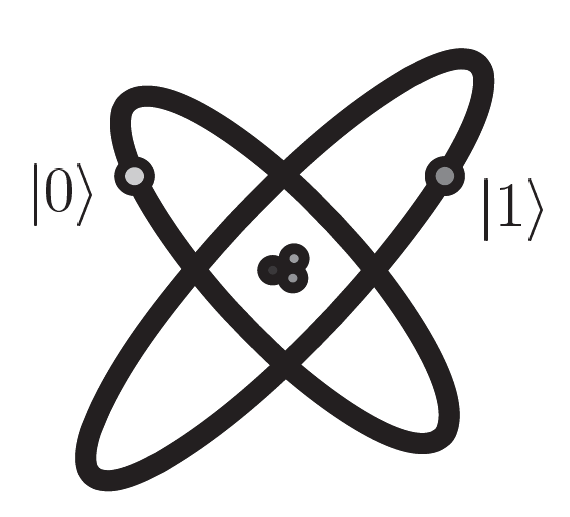
\includegraphics[scale=.4]{atom.png}
	\centering
	\caption{Qubit represented by two electron orbits in an atom, \cite{Nielsen2002}.}
	\label{fig 1.1}
\end{figure}


\section{Postulate 3: Evolution}


The third postulate of quantum mechanics modulates the evolution of a quantum system. That is, the evolution of the state vector that describes the system. In order to properly formalize it, the concepts of eigenvectors, eigenvalues, and Hermitian operators are required.


\subsection{Eigenvalues and eigenvectors}


\begin{definition}
	Let $V$ be a vector space and $A$ an operator on $V$. An \emph{eigenvector} is a non zero vector $|v_\lambda\ra$ such that $A|v_\lambda\ra = \lambda|v_\lambda\ra$ for a complex value $\lambda$ called the associated \emph{eigenvalue}.
\end{definition}

Eigenvalues and their associated eigenvectors will usually be denoted with the same letter for simplicity: $\lambda$ and $|\lambda\ra$. We assume the reader is familiar with eigenvectors and values basic notions. For instance, that they may be calculated using the \emph{characteristic equation}: $|I - \lambda A| = 0$.

\begin{definition}
	A \emph{diagonal representation} of an operator $A$ is a representation $\sum_i \lambda_i |\lambda_i\ra\la\lambda_i|$ where the $|\lambda_i\ra$ form an orthonormal set of A's eigenvectors and $\lambda_i$ are the respective eigenvalues. An operator is said to be \emph{diagonalizable} if it allows a diagonal representation.
\end{definition}

\begin{exampleth}
	As an example of this, let us consider the following matrix:
	
	$$ Z = 
	\begin{pmatrix}
		1 & 0 \\
		0 & -1 
	\end{pmatrix}
	$$
	
	This matrix is called the \emph{Z Pauli} matrix. It is relevant for quantum computing and it will be introduced later on along with the rest of the Pauli matrices. For now, Let's compute its diagonalizable representation. Since it is already diagonal we can infer that its eigenvalues are $\{1, -1\}$. Computing the diagonal representation we realize that a pair orthonormal eigenvectors are $\{|0\ra, |1\ra\}$ respectively. Therefore:
	
	$$ Z = 
	\begin{pmatrix}
		1 & 0 \\
		0 & -1 
	\end{pmatrix} = 
	|0\ra\la0| - |1\ra\la1|
	$$
\end{exampleth}

Normal operators have significant relevancy thanks to the following result:

\begin{theorem}[Spectral Decomposition Theorem]
\label{spectral-decomposition-theorem}
	An operator $A$ is normal if and only if it is diagonalizable.
\end{theorem}
\begin{proof}
	TODO: To be copied, Box 2.2, page 72, Nielsenchen.
\end{proof}

Since Hermitian and unitary operators are normal, it follows the next

\begin{corollary}
	Any Hermitian operator is diagonalizable. Any unitary operator is diagonalizable.
\end{corollary}


\subsection{Postulate 3 statement}

\begin{postulate}
	The evolution of a \emph{closed} quantum system is described by a \emph{unitary transformation}. That is, the state $|\varphi\ra$ of the system at time $t_1$ is related to the state $|\varphi'\ra$ of the system at time $t_2$ by a unitary operator $U$ which depends only on the times $t_1$ and $t_2$,
	
	$$ |\varphi'\ra = U|\varphi\ra $$
\end{postulate}

Just like the first postulate does not provide the state space or state vector of the system, the third postulate does not provide the unitary transformation that concretes this evolution. For our quantum computing case, we will be the ones to define the unitary transformation to the system. That is, the quantum circuit that transforms our qubit.

\begin{exampleth} Let's consider the \emph{X Pauli matrix}, also known as the \emph{bit flip} matrix:
	
	$$ \sigma_1 = X = 
	\begin{pmatrix}
		0 & 1 \\
		1 & 0 
	\end{pmatrix}
	$$
	
	It is called the bit flip matrix because it takes $|0\ra$ to $|1\ra$ and vice-versa:
	
	$$  X|0\ra = 
	\begin{pmatrix}
		0 & 1 \\
		1 & 0 
	\end{pmatrix}
	\begin{pmatrix}
		1 \\
		0 
	\end{pmatrix}=
	\begin{pmatrix}
		0 \\
		1 
	\end{pmatrix} =
	|1\ra
	$$
	
	This product that we just computed is precisely what postulate 3 states: the evolution of our state vector following the unitary operator $X$: $X|0\ra = |1\ra$. Even though for an arbitrary system we do not know the specific unitary transformation the system follows, we can create systems that follow certain desired transformations. These are the basics of quantum gates and quantum circuits. 
\end{exampleth}

The description of the system evolution provided by Postulate 3 only bears information for those fixed times $t_1$ and $t_2$. A continuous time-description of this evolution is provided by the Schrodinger equation, which provides a redefinition of the second postulate.

\begin{postulate 3'}
	The time evolution of the state of a \emph{closed} quantum system is described by the Schrodinger equation:
	
	$$ i \hbar \frac{d|\varphi\ra}{dt} = H|\varphi\ra $$
	
	where $\hbar$ is \emph{Planck’s constant}, $i$ is the imaginary unit and $H$ is a fixed Hermitian operator known as the $Hamiltonian$.
\end{postulate 3'}

There are several notes to make about this postulate. First, the Hamiltonian is fixed for the given system and it is not be confused with the \emph{Hadamard quantum gate}, also represented by an $H$. Second, $\hbar$ is a physical constant that can be absorbed into the Hamiltonian for our purposes, simplifying the equation. Finally, this is a differential equation, so by knowing the initial state space of the system and the exact Hamiltonian we may know the exact evolution of the system.

Let us study the Hamiltonian in general. Since it is a Hermitian operator, it allows a spectral decomposition by theorem \ref{spectral-decomposition-theorem}:

$$ H = \sum_E E |E\ra\la E| $$

where $E$ are the eigenvalues and $|E\ra$ the respective normalized eigenvectors. the states $|E\ra$ are usually referred to as \emph{energy eigenstates} or \emph{stationary states}, and $E$ is the \emph{energy} of the state $|E\ra$. Furthermore, the lowest energy is called the \emph{ground energy state} while the corresponding eigenstate is called the \emph{ground state}.

\begin{exampleth} Suppose a single qubit system has a the following Hamiltonian:
	
	$$ H = \hbar \omega X = \hbar \omega
	\begin{pmatrix}
		0 & 1 \\
		1 & 0 
	\end{pmatrix}
	$$
	
	Where $X$ is the first Pauli matrix, and $\omega$ is a positive parameter. H eigenenergy states are the same as $X$ eigenstates: $(|0\ra + |1\ra)/2$ and $(|0\ra - |1\ra)/2$ with respective energies $\hbar\omega$ and $-\hbar\omega$. Thus, the ground state is $(|0\ra - |1\ra)/2$ with ground state energy $-\hbar\omega$.
\end{exampleth}

Let us deduce the connection between the Hamiltonian perpestive of dinamics, Postulate 3', and the unitary operator perspective, postulate 3. We can solve the Schrodinguer equation, which can be proven to be:

$$ |\varphi(t_2)\ra = \text{exp} \bigg(  \frac{-iH(t_2-t_1)}{\hbar} \bigg) |\varphi(t_1)\ra $$

We define:

$$ U(t_1, t_2) \equiv \text{exp} \bigg(  \frac{-iH(t_2-t_1)}{\hbar} \bigg) $$

Which is a unitary operator. In fact, any unitary operator $U$ may be expressed as $U = \text{exp(iK)}$ for some Hermitian operator $K$. Thus, we obtained: 

$$ |\varphi(t_2)\ra = U(t_1, t_2) |\varphi(t_1)\ra $$

Following this procedure, we have proven that there is a one to one correspondence between the continuous time-varying postulate 3' using the Hamiltonian and the more stationary discrete-time version using the unitary operator. Although the discrete-time vision is usually used in quantum computing, Quantum Annealing -the specific application of quantum mechanics used in this thesis- rests mostly on the Hamiltonian point of view. We will deepen in this architecture on section [TODOref].

It is worth mentioning that both versions of this postulate assume our physical system to be \emph{closed}. That is, there is no interaction with the system coming from the exterior. In reality, the only real closed system is the universe as a whole. However, we may recreate sufficiently closed systems so that they can be described with approximations as being closed. 

Furthermore, this severely interferes with postulate 2, where an outsider to the system may interfere with it by measuring it. The quantum system will evolve following postulate 3 until measurement is applied. Then they will evolve following the behavior described on postulate 2.

In practice, obtaining the Hamiltonian for a given quantum system is a really laborious work and usually needs experimental data [TODO: add evidence? stated as such in Niel.]. However, for our computational purposes, we will be the ones designing the Hamiltonian such that our system evolves as desired. In particular, chapter 3 [TODOref to QUBO chapter] describes in detail the construction of Hamiltonians for QUBO problems.

\subsection{Quantum Computing perspective: Quantum Gates}

Although quantum annealing does not make use of quantum gates, they are the basis of quantum computing and they fully rely on postulate 3. Because of their importance, a brief overview of quantum gates is provided o¡in this section. However, a profound understanding of them will not be necessary to understand the rest of the thesis.

Quantum computing is built upon the most simple operation we can compute on single qubits: quantum gates. Since state vectors are unit two-dimensional vectors, the operations we apply to them must preserve the norm. Thus, quantum gates will be represented by 2x2 unitary matrices. We have already introduce some of the most famous gates, the Pauli matrices:

$$ X =
\begin{pmatrix}
	0 & 1 \\
	1 & 0 
\end{pmatrix}; \quad
Y =
\begin{pmatrix}
	0 & -i \\
	i & 0 
\end{pmatrix}; \quad
Z =
\begin{pmatrix}
	1 & 0 \\
	0 & -1 
\end{pmatrix}
$$

Some of the others most important gates are the Hadamard gate (denoted as H), the phase gate (denoted as S), and the $\pi/8$ gate (denoted as T):

$$ H = \frac{1}{\sqrt 2}
\begin{pmatrix}
	1 & 1 \\
	1 & -1 
\end{pmatrix}; \quad
S =
\begin{pmatrix}
	1 & 0 \\
	0 & i 
\end{pmatrix}; \quad
T =
\begin{pmatrix}
	1 & 0 \\
	0 & e^{i\pi/4} 
\end{pmatrix}
$$

Although we have not described the fundamentals of multiple qubits systems (postulate 4 is required for it), it is worth mentioning a simple two-qubits gate for the purpose of this section. Just like in classical computing, conditional operations are essential for the construction of complex quantum algorithms. The most basic conditional operation is the \emph{controlled-NOT} gate, also referred to as the CNOT gate. This gate takes two bits $|c\ra|t\ra$, a control qubit, and a target qubit. It flips the target qubit if the first qubit is set to $|1\ra$, producing the operation $|c\ra|t\ra \rightarrow |c\ra|c \oplus t\ra$, where $\oplus$ denotes the exclusive-or operation. Therefore, if the control qubit is $|c\ra = \alpha|0\ra + \beta|1\ra$, it will virtually flip the target qubit with probability $|\beta|^2$ and leave it how it is with probability $|\alpha|^2$. We will come back to this gate once we know the formalism of multiple qubits systems.

One of the most important results of classical computation theory is that any boolean function may be constructed by only using AND, OR, and NOT gates, or by simply using NAND gates \cite{Lau2006}. There is an equivalent result concerning quantum gates \cite{Bayens2019}.

\begin{theorem}
	Any unitary matrix can be approximated by a combination of the Hadamard, CNOT, and $\pi/8$ gates.
\end{theorem}

In this case, \{H, CNOT, T\} is called a \emph{universal gate set}. In practice, is it efficient to build such any gate using only this gate set? The answer to the question is positive, as stated by the \textbf{Solovay-Kitaev theorem} \cite{Dawson2006}. However, this is out of the scope of this project. We provide a sketch proof of the previous theorem from \cite{Bayens2019}.

\begin{proof}
	TODO: copy proof from Bayens, Theorem 4.2
\end{proof}

Further study of quantum circuits falls out of the scope of this thesis since we will use the D-Wave architecture, which relies on quantum annealing instead of quantum circuits.

\section{Postulate 4: Composite systems}


In this section, we introduce the last postulate, which lets us understand the state space associated with a physical system composed of other minor systems. This will allow us to study multiple-qubits systems and state some of the most important results in quantum mechanics and quantum computing: The \emph{Heisenberg uncertainty principle} and the no-cloning theorem.


\subsection{Tensor product}


Let $V$ and $W$ be complex vector spaces with dimensions $m$ and $n$ respectively. Then, $V \otimes W$, read '$V$ tensor $W$', is a $mn$ complex vector space. Let $|v\ra$ and $|w\ra$ be vectors in $V$ and $W$ respectively. Then, $|v\ra \otimes |w\ra$ is in $V \otimes W$. Furthermore, any element of $V \otimes W$ may be expressed as a linear combinations of tensor products $|v\ra \otimes |w\ra$ of elements from $V$ and $W$. We may describe elements of $V \otimes W$ using the following equivalent notations: $|v\ra \otimes |w\ra$, $|v\ra|w\ra$, $|v, w\ra$ and even $|vw\ra$.

Let $|i\ra$ and $|j\ra$ be basis for $V$ and $W$ respectively. Then, $|i\ra \otimes |j\ra = |ij\ra$ is a basis for $V \otimes W$. For example, consider the complex vector space $\C^2$. Then

$$ |0\ra \otimes |0\ra + |1\ra \otimes |1\ra = |00\ra + |11\ra $$

is an element in $\C^2 \otimes \C^2 \cong \C^4$ .

Although the tensor product is generally described as an abstract construct, we may provide a more visual perspective using the \emph{Kronecker product}. This is a matrix representation for the tensor product of finite vector spaces. Suppose $A = \{a\}_{ij}$ is a $n \times m$ matrix and $B = \{b\}_{ij}$ is an $p \times q$ matrix. Then $A \otimes B$ is a $np \times mq$, matrix with the following representation:

$$ A \otimes B = 
\begin{pmatrix}
	a_{11}B & a_{12}B & \dotsc & a_{1m}B \\
	a_{21}B & a_{22}B & \dotsc & a_{2m}B \\
	\vdots & \vdots & \vdots & \vdots \\
	a_{n1}B & a_{n2}B & \dotsc & a_{nm}B \\
\end{pmatrix}
$$

For example:

$$ \begin{pmatrix}
	0 & 1 \\
	2 & 3
\end{pmatrix} \otimes
\begin{pmatrix}
	10 & 20 \\
	30 & 40
\end{pmatrix} =
\begin{pmatrix}
	0 \times \begin{pmatrix} 10 & 20 \\ 30 & 40 \end{pmatrix} &
	1 \times \begin{pmatrix} 10 & 20 \\ 30 & 40 \end{pmatrix} \\
	2 \times \begin{pmatrix} 10 & 20 \\ 30 & 40 \end{pmatrix} &
	3 \times \begin{pmatrix} 10 & 20 \\ 30 & 40 \end{pmatrix}
\end{pmatrix} = 
$$
$$ 
\begin{pmatrix}
	0 \times 10 & 0 \times 20 & 1 \times 10 & 1 \times 20 \\
	0 \times 30 & 0 \times 40 & 1 \times 30 & 1 \times 40 \\
	2 \times 10 & 2 \times 20 & 3 \times 10 & 3 \times 20 \\
	2 \times 30 & 2 \times 40 & 3 \times 30 & 3 \times 40
\end{pmatrix} = 
\begin{pmatrix}
	0 & 0 & 10 & 20 \\
	0 & 0 & 30 & 40 \\
	20 & 40 & 30 & 60 \\
	60 & 80 & 90 & 120
\end{pmatrix}
$$

By definition, the tensor product satisfies:

\begin{itemize}
	\item Let $\alpha$ be a complex number. For any $|v\ra$ in $V$ and $|w\ra$ in $W$,
	$$ \alpha(|v\ra \otimes |w\ra) = (\alpha|v\ra) \otimes |w\ra = |v\ra \otimes (\alpha|w\ra) $$
	
	\item For any $|v_1\ra$, $|v_2\ra$ in $V$ and $|w\ra$ in $W$,
	$$ (|v_1\ra + |v_2\ra) \otimes |w\ra = |v_1\ra \otimes |w\ra + |v_2\ra \otimes |w\ra $$
	
	\item For any $|v\ra$ in $V$ and $|w_1\ra$, $|w_2\ra$ in $W$,
	$$ |v\ra \otimes (|w_1\ra + |w_2\ra) = |v\ra \otimes |w_1\ra + |v\ra \otimes |w_2\ra $$
\end{itemize}

The inner products of the spaces $V$ and $W$ may be use to extend and natural inner product the tensor space. Define:

$$ \bigg ( \sum_i a_i |v_i\ra \otimes |w_i\ra, \sum_j b_j |v_j'\ra \otimes |w_j'\ra \bigg ) \equiv
		\sum_{ij} \overline{a_i} b_j \la v_i|v_j' \ra \la w_i|w_j' \ra $$

With this product and the previous properties in mind, it can easily be proven that the tensor product of Hilbert spaces is a Hilbert space.

\begin{proposition}
	Let $H_1$ be and $H_2$ be two Hilbert spaces with respective orthonormal bases $B_1 = \{|v_i\ra\}_{i=1,\dots,n}$ and $B_2 = \{|w_j\ra\}_{j=1,\dots,m}$. Then, $H_1 \otimes H_2$ is a Hilbert space with inner product given by
	
	$$ ( |v\ra \otimes |w\ra, |v'\ra \otimes |w'\ra) = \la vw|v'w'\ra = \la v|v'\ra\la w|w'\ra $$
	
	For any $|v\ra, |v'\ra$ in $V$ and $|w\ra, |w'\ra$ in $W$. Furthermore, $B_1 \otimes B_2 = \{|v_i w_j\ra\}_{i,j}$ is an orthonormal basis of $H_1 \otimes H_2$.
\end{proposition}

\begin{proof}
	By definition, $H_1 \otimes H_2$ is a complex vector space with $dim(H_1 \otimes H_2) = dim(H_1) \cdot dim(H_2)$. Furthermore, $B_1 \otimes B_2 = \{|v_i\ra \otimes |w_j\ra\}_{i,j} = \{|v_i w_j\ra\}_{i,j}$ is a base of it. Let $|v_i w_j\ra, |v_k w_l\ra \in B_1 \otimes B_2$:
	
	$$ \la v_i w_j|v_k w_l \ra = \la v_i|v_k \ra \la w_j|w_l \ra = \delta_{ik} \delta_{jl} $$
	
	which equals one if and only if $i = k$ and $j = l$, and zero otherwise. Thus, proving that $B_1 \otimes B_2$ is orthonormal.
	
	Finally, for $H_1 \otimes H_2$ to be a Hilbert space the product defined above needs to be, in fact, an inner product. It suffies to prove that it is definite positive. Let $|v\ra \in H_1 \otimes H_2$. Since $B_1 \otimes B_2$ is an orthonormal basis, there exist $\alpha_{ij} \in \C$ such that:
	
	$$ |v\ra = \sum_{i,j} \alpha_{ij} |v_i w_j\ra $$
	
	By linearity:
	
	$$ \la v|v \ra = \sum_{i,j,k,l} \overline{\alpha_{ij}} \alpha_{kl} \la v_i w_j|v_k w_l \ra = \sum_{i,j,k,l} \overline{\alpha_{ij}} \alpha_{kl} \  \delta_{ik} \delta_{jl} = \sum_{i,j} |\alpha_{ij}|^2  \geq 0 $$
	
	where the equality holds if and only if $\alpha_{ij} = 0 \ \forall i,j$.
\end{proof}

From the inner product, the tensor space $H_1 \otimes H_2$ naturally inherits the notions of adjoint, unitary, normality and Hermicity. We will denote a vector $|\varphi\ra$ tensored with itsel n times, $|\varphi\ra \otimes \overplace{n}{\dotsc} \otimes |\varphi\ra$, as $|\varphi\ra^{\otimes n}$, and equivalently with Hilbert spaces: $H \otimes \overplace{n}{\dotsc} \otimes H$, as $H^{\otimes n}$. For our quantum computing purposes, the following case holds particular relevance.

\begin{corollary}
	The tensor product of $\C^2$ with itself n times, $\C^2 \otimes \overplace{n}{\dotsc} \otimes \C^2$, is isomorphic to $\C^{2^n}$.
\end{corollary}

\begin{proof}
	Let $H = \C^2 \otimes \overplace{n}{\dotsc} \otimes \C^2$. Since $dim(H) = dim(\C^2)^n = 2^n$, $H$ is a Hilbert space with dimension $2^n$. Thus, by Hausdorff's Theorem \cite{Paya2020}, it is isomorphic to the canonical complex vector space of dimension $2^n$, $\C^{2^n}$.
\end{proof}

In the same way that the inner product was naturally extended to the tensor space, we may extend operators ensuring linearity. Let $A: V \longrightarrow V'$ and $B: W \longrightarrow W'$ two operators between Hilbert spaces. Then, we define $A \otimes B: V \otimes W \longrightarrow V' \otimes W'$ using the following equation:

$$ (A \otimes B)(|v\ra \otimes |w\ra) \equiv A|v\ra \otimes B|w\ra $$

We extend this definition to every element of $V \otimes W$ ensuring linearity:

$$ (A \otimes B) \bigg(\sum_i a_i |v_i\ra \otimes |w_i\ra \bigg) \equiv \sum_i a_i A|v_i\ra \otimes B|w_i\ra $$

It can be shown that $A \otimes B$ is a well-defined linear operator. In fact, any linear operator mapping $V \otimes W$ to $V' \otimes W'$ may be expressed as a linear combination of tensor product of linear operators mapping $V$ to $V'$ and $W$ to $W'$:

$$ C = \sum_i a_i A_i \otimes B_i $$

where by definition:

$$ \bigg( \sum_i a_i A_i \otimes B_i \bigg)|v\ra \otimes |w\ra = \sum_i a_i A_i|v\ra \otimes B_i|w\ra $$


\subsection{Postulate 4 statement}


Reaching the core of this section, suppose we consider two (or more) distinct physical systems. In order to describe the state of the composite system we need to make use of tensor product.

\begin{postulate}
	The state space of a composite physical system is the tensor product of the state spaces of the component physical systems. Moreover, if we have systems numbered $1$ through $n$, and system number $i$ is prepared in the state $|\varphi_i\ra$, then the joint state of the total system is $|\varphi_1\ra \otimes \dotsc \otimes |\varphi_n\ra$.
\end{postulate}

Let us provide an intuitive notion of why is the tensor product used in order to describe composite systems. After all, we would expect that there exists a \emph{somehow canonical way} os describing the product composition of systems, just like the cartesian product is used with vector spaces. Let us refer again to the so-called \emph{superposition principle of quantum mechanics}. Let $|\varphi\ra$ and $|\psi\ra$ be two vector states of a system. Then, any superposition of the states, $\alpha|\varphi\ra + \beta|\psi\ra$, should also be another vector state, where $|\alpha|^2 + |\beta|^2 = 1$. Suppose we now have two systems $X$ and $Y$, with two vector states $|\varphi_x\ra$ and $|\varphi_y\ra$. Then, we could describe the state of the composite system $XY$ as some state $|\varphi_x\ra|\varphi_y\ra$. Studying the superposition principle on composite systems leads us naturally to the notion of tensor product. It is important to note that this development is not thorough, since we are not taking the superposition principle as a fundamental component of our description of quantum mechanics. It does help up to build an intuitive notion on why this tensor product is used.

We now introduce the \emph{Bell State} or \emph{EPR pair:}

$$ |+\ra = \frac{ |00\ra + |11\ra }{ \sqrt 2 } $$

Although it may seem harmless at first glance, this state has been responsible for many surprises during the development of quantum physics \cite{Bellt1964}. Let us have a first look into it, although we will come back to it in section [TODOref seccion de la EPR Paradox].

The first thing to notice about this state is that it can be expressed as a single tensor product of state vector: $|+\ra \neq |a\ra|b\ra$. This means that this state is not describing two independent physical systems put together with their respective vector states independently, it describes a \textbf{relation} between both systems too. It means that those systems are somehow interfering with each other. So we may affect one by disrupting the other.

This phenomenon is called \emph{entaglement}. A state is called \emph{entangled} when it cannot be expressed as the product of states of its component systems. This concept rests at the heart of the disparity between classic physics and quantum physics and it is key in quantum computing. It was deeply studied first by Einstein, Podolsky, and Rosen (EPR) \cite{Einstein1935} and second by John Bell \cite{Bellt1964}.


\subsection{Projective measurement}
\label{projective-measurement}


In this section, we explain an important particular case of measurement. In fact, this method of projective measurement is equivalent to Postulate 2, when they are combined with the capacity to perform unitary operations. It has huge relevancy in quantum computing and it is explained here because of its relation with composite systems. Let us state the alternative postulate:

\begin{postulate 2'}
	A projective measurement is described by an \emph{observable}, $M$, a Hermitian operator on the state space of the system being described. The observable has a spectral decomposition:
	
	$$ M = \sum_m m P_m$$
	
	where $P_m$ is the projector onto the eigenspace with eigenvalue $m$. The possible outcomes of the measurement correspond to the eigenvalues, $m$, of the observable. Upon measuring the state $|\varphi\ra$, the probability of the result $m$ ocurring is:
		
	$$ p(m) = \la \varphi | P_m | \varphi \ra $$
	
	and the state of the system after the measurement, givent that outcome $m$ ocurred, is:
	
	$$ \frac{P_m |\varphi\ra}{\sqrt{p(m)}} $$
\end{postulate 2'}

Projective measurements can be seen as a particular case of Postulate 2. Suppose the measurement operators from such postulate, in addition to satisying the completeness relation $\sum_m M_m M_m^\dagger = I$, also fulfill that $M_m$ are \emph{orthogonal projectors}. That is, $M_m$ is Hermitian and $M_m M_{m'} = \delta_{mm'} M_m \ \forall m,m'$. With these aditional restricions it holds that $M_m M_m^\dagger = M_m M_m = M_m$. By choosing $P_m = M_m$ we see that projective measurements is a particular case of Postulate 2.

Thanks to the way projective measurements are expressed, they have nice and handy properties. Let us compute the average value of a projective measurement:

\begin{equation}
	\begin{split}
		E(M)	& = \sum_m m p(m) \\
				& = \sum_m m \la \varphi | P_m | \varphi \ra \\
				& = \la \varphi | \bigg( \sum_m m P_m \bigg) | \varphi \ra \\
				& = \la \varphi | M | \varphi \ra
	\end{split}
\end{equation}

The average value of an operator is usually written as $\la M \ra \equiv \la \varphi | M | \varphi \ra$. The standar deviation associated to observations of $M$ is then written as:

\begin{equation}
	\begin{split}
	[\Delta(M)]^2	& = \big\la (M - \la M \ra )^2 \big\ra\\
					& = \la M^2 \ra - \la M \ra^2
	\end{split}
\end{equation}

This means that if we prepare our state $|\varphi\ra$ multiple times and measure it, the measures will follow a normal distribution with expected value $\la M \ra$ and standard deviation $\Delta(M) = \sqrt{\la M^2 \ra - \la M \ra^2}$. This formulation of standard deviation using observables provides us with an elegant proof of perhaps the most famous quantum mechanics result: The \emph{Heisenberg uncertainty principle}. Such proof can be found in annex [TODOref anexo con la demostracion, copy from Box 2.4 in Niel.].

There are two additional notations worth mentioning regarding projective measurement. Instead of providing an observable $M$, we will sometimes provide a complete set of orthogonal projectors. That is, a set $P_m$ such that $\sum_i P_m = I$ and $P_m P_{m'} = \delta_{mm'} P_m$. The corresponding implicit observable used in this case is $M = \sum_m m P_m$. Finally, another widely used notation is to 'measure in a basis $|m\ra$', where $|m\ra$ form an orthonormal basis. This simply means that the chosen projectors are  $P_m = |m \ra\la m|$ and the observable is $M = \sum_m m |m \ra\la m|$. This is the usual notation in quantum computing.


\subsection{Quantum Computing perspective: Multiple qubits}


Suppose we have a pair of qubits. In the classical case, two bits can be in four possible states: 00, 01, 10, and 11. Similarly, the two qubits computational basis states are $|00\ra$, $|01\ra$, $|10\ra$ and $|11\ra$. We arrive at this natural notation by knowing that each qubit has $\C^2$ as their associated state space and using the tensor product. Just like in the single qubit case, our two qubits system may be in a superposition of these four states:

$$ |\varphi\ra = \alpha_{00} |00\ra + \alpha_{01} |01\ra + \alpha_{10} |10\ra + \alpha_{11} |11\ra $$

Correspondingly, the measurement of this system will result in either 00, 01, 10 or 11 since we are using the observable $\sum_{x \in \{0,1\}^2} x |x\ra\la x|$, where $\{0,1\}^2$ are the strings of length two where each character is either $0$ or $1$. In fact, it will yield state $x$ with probability $|\alpha_x|^2$, being $\alpha_x$ the coefficient associated with the state $|x\ra$. The condition of the probabilities adding up to one is also called the \emph{normalization condition} and can be expressed as $\sum_{x \in \{0,1\}^2} |\alpha_x|^2 = 1$ for the two qubits case.

The fundamental differences with the single qubit case start on measurement. Of course, we can measure both qubits at the same time, but we could also measure only one of them. In order to achieve this we can use the projectors $P_0 = |00\ra\la00| + |01\ra\la01|$ and $P_1 = |10\ra\la10| + |11\ra\la11|$. Upon measuring, the system will collapse to $P_0|\varphi\ra / \sqrt{p_0}$ with probability:

$$ p_0 = \la\varphi|P_0|\varphi\ra = |\alpha_{00}|^2 + |\alpha_{01}|^2 $$

Since these are the coefficients associated with the first qubit being $0$, this is the probability of first qubit being 0. Furthermore, our system will collapse to:

$$ |\varphi'\ra = \frac{ \alpha_{00} |00\ra + \alpha_{01} |01\ra }{ \sqrt{|\alpha_{00}|^2 + |\alpha_{01}|^2} } $$

Note the normalization term $\sqrt{|\alpha_{00}|^2 + |\alpha_{01}|^2}$, which appears so the post-measurement state still satisfies the normalization condition. Naturally, after obtaining $0$ in the first qubit we can still obtain either $0$ or $1$ in the second qubit, with probabilities 

$$ \frac{ |\alpha_{00}|^2 }{ |\alpha_{00}|^2 + |\alpha_{01}|^2 }  \ \text{ and } \ 
\frac{ |\alpha_{01}|^2 }{ |\alpha_{00}|^2 + |\alpha_{01}|^2 } $$

respectively, adding up to $1$. Correspondingly, the first qubit being measured will yield $1$ with probability $p_1 = |\alpha_{10}|^2 + |\alpha_{11}|^2$.

Additionally, the first qubit independently should satisfy the normalization condition. That is, its probabilities of being $0$ and $1$ upon measurement must add up to $1$. But those are $p_0$ and $p_1$, which add up to one because of the normalization condition for $|\varphi\ra$, as expected.

Let us come back to the previously introduced \emph{Bell State}:

$$ |+\ra = \frac{ |00\ra + |11\ra }{ \sqrt 2 } $$

When measuring using the previously defined projectors $P_0$ and $P_1$ we obtain that the first qubit will collapse to either 0 or 1 with equal probability $p_0 = p_1 = 1/2$. Most importantly, in the first case the qubit will collapse to the state:

$$ \frac{ |00\ra / \sqrt 2 }{ \sqrt p_0 } = |00\ra $$

Meaning that the second qubit also collapsed to 0. Note that we only affected the first qubit and the second one was disturbed. These are the consequences of entanglement, key in the appearance of impressive results such as the EPR Paradox [TODOref EPR paradox].

Let us finally consider the more general case. In an n-qubits system our computational (orthonormal) basis would consist of the sates $|x_1 x_2 \dotsc x_n\ra$, where $x_i \in \{0,1\}$. As we already know, in a single qubit system we have two amplitudes $\alpha_0$ and $\alpha_1$. We have four amplitudes for a 2-qubits system, eight for a 3-qubits system... And $2^n$ for an n-qubits system. This means that the number of amplitudes grows exponentially as we add qubits to the system. An immense increment compared to the classical case where the quantity of information that our system holds grows linearly with the numbers of bits. Of course, it is not that simple, since there are huge limitations on how we may access this information in the quantum realm such as how a qubit collapses upon measurement and the no-cloning theorem. However, we can already glimpse the power of quantum computing versus the classical one.


\section{The no-cloning theorem}


A first exposure to the basis of quantum computing is fundamentally incomplete without the no-cloning theorem. It lets us understand one of the fundamental inconveniences of quantum computing: the impossibilty of cloning arbitrary states.

We proceed by formalizing the copying mechanism. Let $H$ be a state space and $|\varphi\ra \in H$ the state to be copied. Given another state $|\varphi'\ra \in H$, we would like to copy $|\varphi\ra$ into $|\varphi'\ra$. Since we can prepare $|\varphi'\ra$ at will before the copying occurs, let  $|\varphi'\ra = |x_0\ra$ be a fixed state. Then, our copying operation will take both states and produce the following result:

$$ (|\varphi\ra \otimes |x_0\ra) \xrightarrow{U} |\varphi\ra \otimes |\varphi\ra $$

Operations between n-qubits (n-qubits gates) must preserve their norm, thus they must be unitary $n \times n$ matrices. In our case, $U$ is a $2 dim(H) \times 2 dim(H)$ unitary matrix. Let us now state and prove the theorem.

\begin{theorem}[No-cloning Theorem]
\label{no-cloning-theorem}
	There is no unitary operator $U: H^{\otimes 2} \longrightarrow H^{\otimes 2}$ and state $|x_0\ra \in H$ such that for any arbitrary state $|\varphi\ra \in H$ it holds
	
	$$ U |\varphi\ra |x_0\ra = |\varphi\ra |\varphi\ra $$
\end{theorem}
\begin{proof}
	Suppose there exists such unitary operator $U$ and such state $|x_0\ra$. Let $|\varphi\ra, |\psi\ra \in H$. We may apply the copying operators to both of them:
	
	$$ U |\varphi\ra |x_0\ra = |\varphi\ra |\varphi\ra $$
	$$ U |\psi\ra |x_0\ra = |\psi\ra |\psi\ra $$
	
	Taking the inner product of both equations and using that $U$ is unitary results in:
	
	\begin{equation*}
		\begin{gathered}
			\bigg( U |\varphi\ra |x_0\ra, U |\psi\ra |x_0\ra \bigg) = \bigg( |\varphi\ra |\varphi\ra, |\psi\ra |\psi\ra \bigg) \iff \\
			\bigg( |\varphi\ra |x_0\ra, |\psi\ra |x_0\ra \bigg) = \la\varphi|\psi\ra \la\varphi|\psi\ra \iff \\
			\la\varphi|\psi\ra \la x_0|x_0 \ra = \la\varphi|\psi\ra^2
		\end{gathered}
	\end{equation*}
	
	Since $|x_0\ra$ is a normalized vector, $\la x_0|x_0 \ra = 1$, and we obtain:
	
	$$\la\varphi|\psi\ra = \la\varphi|\psi\ra^2$$
	
	Which only holds if $\la\varphi|\psi\ra$ equals to either $0$ or $1$, which means $|\varphi\ra$ and $|\psi\ra$ are either equal or orthonormal. But those vectors were arbitrary, thus such a general cloning operator is impossible. 
\end{proof}

TODO: Creo que me gustaría añadir aquí una sección sobre la EPR Paradox / teleportación cuántica.




TODO: CNOT gate explained
TODO: tabular los postulados
TODO: Eliminar todos los Let's



